\section{Performance Vergleich}
\label{sec:Performance Vergleich}

\subsection{Testaufbau}
Zwei Desktop-Rechner der HSR, mit je 16GB Ram und Intel Xeon 3.4Ghz Quad-Core CPUs, sind via Gigabit-Lan miteinander verbunden. Auf den Rechnern läuft Ubuntu 14.04 x64 sowie jPerf und die jeweils getestete Software.

%Semantics, Grafik evtl. noch anpassen das jPerf und Applikation auf Deutsch.
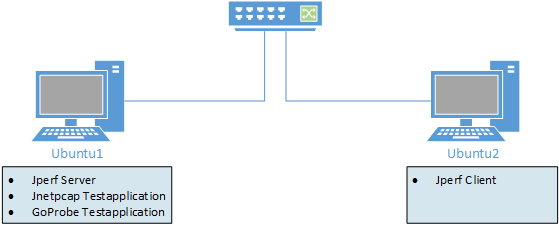
\includegraphics[width=0.7\textwidth]{start/img/PerformanceEvaluation.png}
%todo kontrollieren das Quadcore und nicht Ocata-Core.

\subsection{Testdurchführung}
Auf einem der beiden Rechnern läuft jeweils jPerf im Server-Modus sowie die getestete Software. Auf dem anderen Computer läuft jPerf im Client-Modus.
Via. jPerf wird nun soviel Traffic erzeugt um die 1Gbit/s-Leitung möglichst stark auszulasten, d.h. durchschnittlich 900mbit/s. Die getestete Software zeichnet dabei die ganzen Pakete auf und sollte dabei 300mbit/s an Traffic ertragen können. 300mbit/s sind gem. Open Systems AG die Lastspitzen mit denen etwa zu rechnen sind.

\subsection{Ergebnisse}
Sowohl mit JNetPcap auf Java als auch mit goProbe auf Golang lassen sich mehr als 300mbit/s an Verkehr aufzeichnen. GoProbe ist mit den Durchschnittlich 16\% CPU Auslastung aber etwas performanter als JNetPcap. Die 31\% CPU Lastspitze beim Java Programm gibt es jeweils nur wenn das Programm zum ersten Mal gestartet wird und kommt daher dass dann zuerst eine \acs{JVM} hochgefahren werden muss.
Beim Speicherverbrauch hat goProbe aber deutlich die Nase vorne. So wird tatsächlich nur ein Bruchteil des physischen Speichers (RES) gegenüber Java verwendet.

%TODO: RES evtl. noch verlinken.

\begin{table}[h]
\begin{tabular}{|l|l|l|l|l|l|l|}
\hline
\rowcolor[HTML]{C0C0C0} 
\textbf{Software} & \textbf{CPU Top} & \textbf{CPU Ø} & \textbf{Mem Ø} & \textbf{VIRT\footnotemark[1]} & \textbf{RES\footnotemark[2]} & \textbf{SHR\footnotemark[3]} \\ \hline
JNetPcap          & 31\%             & 20\%           & 0.9\%          & 7030296kb       & 147840kb       & 19588kb        \\ \hline
goProbe           & 18\%             & 16\%           & 0.3\%          & 315268kb        & 1964kb         & 1676kb         \\ \hline
\end{tabular}
\end{table}

\footnotetext[1]{VIRT steht für die virtuelle Grösse eines Prozesses.}
\footnotetext[2]{RES steht für den tatsächlich, physisch verbrauchten Hauptspeicher.}
\footnotetext[3]{SHR zeigt wie viel von VIRT mit anderen Prozessen teilbar ist. Dazu gehören z.B. Shared Libraries.}